\chapter{Fundamentação Teórica}
\label{cap:fundamentacao-teorica}
%\phantom{0}

Neste capítulo são detalhados os tópicos necessários para compreensão das técnicas usadas na elaboração do método proposto. As seções a seguir abordam conceitos sobre o exame de TC, o rim e tumores renais, aprendizado profundo e as métricas de desempenho para validar os resultados experimentais.

\section{Rins e Tumores Renais}
\label{sec:rins-e-tumores-renais}

Os rins são órgãos bilaterais em forma de feijão, de cor marrom-avermelhada e localizados na região posterior do abdômen. Geralmente, o rim direito é ligeiramente menor e mais baixo que o esquerdo devido à presença do fígado. Cada rim pesa cerca de 125-170 gramas nos homens e 115-155 gramas nas mulheres, e são revestidos por uma cápsula renal fibrosa e resistente. Além disso, duas camadas de gordura servem como proteção \cite{tim_newman}.

\begin{figure}[!ht]
    \centering
    \caption{Estrutura interna do rim.}
    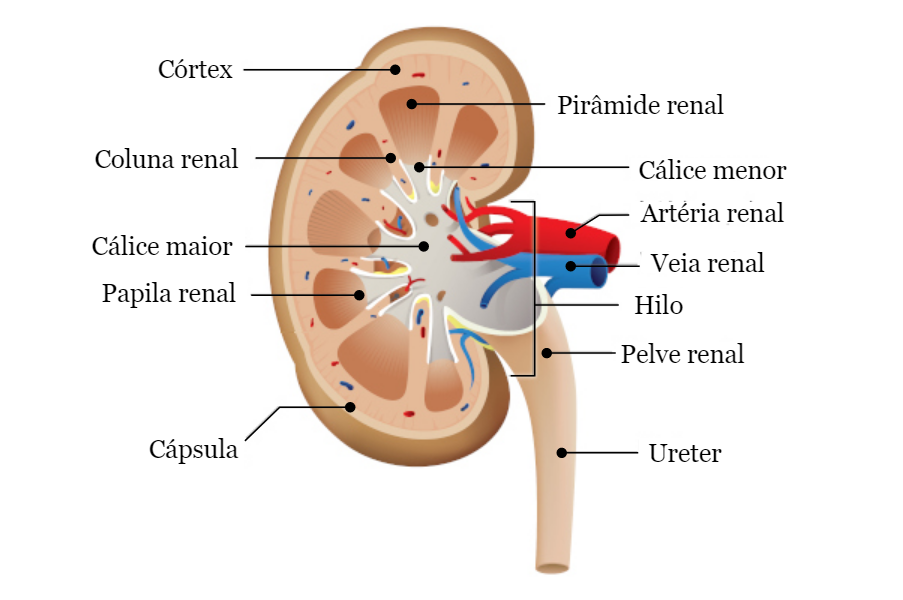
\includegraphics[width=0.85\textwidth]{figuras/anatomia-rins-interno.png}
    \legend{Fonte: \cite{vanessa_sardinha}.}
    \label{fig:anatomia-rins-interno}
\end{figure}


A maioria dos casos de câncer renal tem cura com um diagnóstico precoce. Para iniciar o tratamento adequado do câncer renal, a segmentação acurada dos rins é necessária. Portanto, as informações estruturais do rim são analisadas por meio de exames de ultrassom, Ressonância Magnética (RM) ou TC de abdômen. Embora as imagens RM tenham sido usadas para segmentação renal em alguns estudos na literatura~\cite{goceri2011automatic,7424483}, a TC, dentre as modalidades disponíveis, é considerada o padrão ouro, especialmente para o diagnóstico de câncer precoce~\cite{kaur2016survey}. Além disso, a TC é muito útil no estadiamento (verificação da extensão para outros órgãos) e no planejamento terapêutico.

\section{Tomografia Computadorizada}
\label{sec:tumografia-computadorizada}

Para planejar o tratamento radioterápico, é necessário obter informações sobre os tumores renais, como tamanho e a localização exata. Para isso, é necessária uma imagem tridimensional detalhada da região do abdômen do paciente, geralmente realizada por meio do exame de TC. Essas informações são eventualmente usadas para orientar o radioterapeuta a produzir o melhor tratamento radioterápico para cada paciente.



\section{Processamento Digital de Imagens}
\label{sec:processamento-digital-imagens}

O processamento digital de imagens é definido como um conjunto de técnicas computacionais que transformam uma imagem de entrada em uma saída desejada~\cite{gonzalez2008digital}. Esse conjunto de técnicas permite extrair e identificar informações de imagens e melhorar a qualidade visual de aspectos estruturais, facilitando a percepção humana e a interpretação automática por meio de máquinas~\cite{pedrini2008analise}.

Existem vários algoritmos com propósitos muito específicos, que juntos formam a metodologia final. Portanto, uma metodologia difere de outra na forma como compõe suas etapas ou ferramentas, mas normalmente segue as etapas apresentadas por \citeonline{gonzalez2008digital}:

\begin{enumerate}
    \item Aquisição das imagens: as imagens são capturadas por meio de um dispositivo ou sensor e transformadas em um formato que pode ser processado posteriormente. Porém, como resultado desse processo, a imagem resultante pode apresentar falhas devido às condições de iluminação ou às características do dispositivo, por exemplo;
    
    \item Pré-processamento: o objetivo é melhorar a qualidade da imagem por meio de técnicas para reduzir o ruído, realçar o contraste e suavizar certas estruturas da imagem;
    
    \item Segmentação: consiste em localizar e extrair áreas de interesse contidas na imagem, com o objetivo de dividir a imagem isolando os diferentes objetos que a compõem;
    
    \item Representação e descrição: denominada de extração de características, pois extrai informações que podem ser usadas para discriminar classes de objetos;
    
    \item Reconhecimento e interpretação: reconhecimento é o processo que atribui um identificador aos objetos da imagem. A interpretação consiste em atribuir um significado ao conjunto de objetos reconhecidos.
\end{enumerate}



\begin{equation}
\label{eq:relu}
\sigma(x) = max(0,x),
\end{equation}
\begin{equation}
\label{eq:leakyrelu}
\sigma(x) = max(0.1,x).
\end{equation}

\subsection{Redes \textit{Multilayer Percepton}}
\label{sec:redes-multilayer-percepton}



\begin{figure}[!ht]
    \centering
    \caption{Rede \textit{Multilayer Percepton}.}
    
\includegraphics[width=0.45\textwidth]{figuras/RNA.png}
    \legend{Fonte: Elaborado pela autora.}
    \label{fig:rna}
\end{figure}



\section{Considerações Finais}
\label{consideracoes-finais-fundamentacao}

Neste capítulo, foi apresentada a fundamentação teórica necessária para a compreensão das técnicas utilizadas e suas aplicações no método proposto. Foram abordados temas como: rins e tumores renais, exame de TC, técnicas de pré-processamento digital de imagens, aprendizado profundo e métricas de desempenhos.